% Springer LNCS. Download llncs.cls from Springer (or use the Overleaf "Springer LNCS" template)
% and place it next to this file.  All result numbers come from generated/numbers.tex.
\IfFileExists{llncs.cls}{\documentclass[runningheads]{llncs}}{%
  % fallback so the draft compiles without llncs.cls (layout differs from the final)
  \documentclass[10pt]{article}\usepackage[margin=1in]{geometry}
  \newcommand{\institute}[1]{}\newcommand{\titlerunning}[1]{}\newcommand{\authorrunning}[1]{}
  \newcommand{\keywords}[1]{\par\noindent\textbf{Keywords:} ##1}\renewcommand{\and}{\unskip, }}
\usepackage[T1]{fontenc}
\usepackage{graphicx,booktabs,amsmath,amssymb,hyperref,xcolor}
% AUTO-GENERATED by scripts/make_tables.py -- do not edit by hand
% source: results/merged
\newcommand{\NCertOne}{5}
\newcommand{\NCertTwo}{5}
\newcommand{\NCertThree}{4}
\newcommand{\NCertFour}{1}
\newcommand{\NCertFive}{0}
\newcommand{\NModels}{25}
\newcommand{\NCertified}{15}
\newcommand{\RelMSEMax}{0.0030}
\newcommand{\EtoEAccMin}{1.000}
\newcommand{\MaxConservationErr}{6.9e-06}
\newcommand{\DfeatCLTDOne}{1.00}
\newcommand{\DfeatLoCLTDOne}{1.00}
\newcommand{\DfeatHiCLTDOne}{1.00}
\newcommand{\DCRCLTDOne}{1.00}
\newcommand{\SkipCLTDOne}{0.00}
\newcommand{\DirectCLTDOne}{0.14}
\newcommand{\DfeatPLTDOne}{1.00}
\newcommand{\DfeatLoPLTDOne}{1.00}
\newcommand{\DfeatHiPLTDOne}{1.00}
\newcommand{\DCRPLTDOne}{1.00}
\newcommand{\SkipPLTDOne}{0.00}
\newcommand{\DirectPLTDOne}{0.14}
\newcommand{\DfeatPLTpmDOne}{1.00}
\newcommand{\DfeatLoPLTpmDOne}{1.00}
\newcommand{\DfeatHiPLTpmDOne}{1.00}
\newcommand{\DCRPLTpmDOne}{1.00}
\newcommand{\SkipPLTpmDOne}{0.00}
\newcommand{\DirectPLTpmDOne}{0.14}
\newcommand{\DfeatCLTDTwo}{1.50}
\newcommand{\DfeatLoCLTDTwo}{1.43}
\newcommand{\DfeatHiCLTDTwo}{1.58}
\newcommand{\DCRCLTDTwo}{0.75}
\newcommand{\SkipCLTDTwo}{0.19}
\newcommand{\DirectCLTDTwo}{0.12}
\newcommand{\DfeatPLTDTwo}{1.46}
\newcommand{\DfeatLoPLTDTwo}{1.39}
\newcommand{\DfeatHiPLTDTwo}{1.52}
\newcommand{\DCRPLTDTwo}{0.73}
\newcommand{\SkipPLTDTwo}{0.14}
\newcommand{\DirectPLTDTwo}{0.12}
\newcommand{\DfeatPLTpmDTwo}{1.43}
\newcommand{\DfeatLoPLTpmDTwo}{1.37}
\newcommand{\DfeatHiPLTpmDTwo}{1.49}
\newcommand{\DCRPLTpmDTwo}{0.71}
\newcommand{\SkipPLTpmDTwo}{0.14}
\newcommand{\DirectPLTpmDTwo}{0.11}
\newcommand{\DfeatCLTDThree}{1.93}
\newcommand{\DfeatLoCLTDThree}{1.89}
\newcommand{\DfeatHiCLTDThree}{1.97}
\newcommand{\DCRCLTDThree}{0.64}
\newcommand{\SkipCLTDThree}{0.38}
\newcommand{\DirectCLTDThree}{0.04}
\newcommand{\DfeatPLTDThree}{1.97}
\newcommand{\DfeatLoPLTDThree}{1.93}
\newcommand{\DfeatHiPLTDThree}{2.01}
\newcommand{\DCRPLTDThree}{0.66}
\newcommand{\SkipPLTDThree}{0.27}
\newcommand{\DirectPLTDThree}{0.04}
\newcommand{\DfeatPLTpmDThree}{1.94}
\newcommand{\DfeatLoPLTpmDThree}{1.87}
\newcommand{\DfeatHiPLTpmDThree}{2.00}
\newcommand{\DCRPLTpmDThree}{0.65}
\newcommand{\SkipPLTpmDThree}{0.27}
\newcommand{\DirectPLTpmDThree}{0.05}
\newcommand{\DfeatCLTDFour}{2.03}
\newcommand{\DfeatLoCLTDFour}{2.03}
\newcommand{\DfeatHiCLTDFour}{2.03}
\newcommand{\DCRCLTDFour}{0.51}
\newcommand{\SkipCLTDFour}{0.48}
\newcommand{\DirectCLTDFour}{0.05}
\newcommand{\DfeatPLTDFour}{2.01}
\newcommand{\DfeatLoPLTDFour}{2.01}
\newcommand{\DfeatHiPLTDFour}{2.01}
\newcommand{\DCRPLTDFour}{0.50}
\newcommand{\SkipPLTDFour}{0.33}
\newcommand{\DirectPLTDFour}{0.05}
\newcommand{\DfeatPLTpmDFour}{2.00}
\newcommand{\DfeatLoPLTpmDFour}{2.00}
\newcommand{\DfeatHiPLTpmDFour}{2.00}
\newcommand{\DCRPLTpmDFour}{0.50}
\newcommand{\SkipPLTpmDFour}{0.31}
\newcommand{\DirectPLTpmDFour}{0.05}
\newcommand{\DiffCLTPLTDOne}{0.00}
\newcommand{\PvalDOne}{1.000}
\newcommand{\DiffCLTPLTDTwo}{0.04}
\newcommand{\PvalDTwo}{0.125}
\newcommand{\DiffCLTPLTDThree}{-0.04}
\newcommand{\PvalDThree}{0.125}
\newcommand{\DiffCLTPLTDFour}{0.02}
\newcommand{\PvalDFour}{1.000}
\newcommand{\TrendRhoCLT}{0.97}
\newcommand{\TrendPCLT}{1.54e-09}
\newcommand{\TrendRhoPLT}{0.97}
\newcommand{\TrendPPLT}{1.54e-09}
\newcommand{\TrendRhoPLTpm}{0.97}
\newcommand{\TrendPPLTpm}{1.54e-09}
\newcommand{\SlopeDiffCLTminusPLT}{0.01}
\newcommand{\SkipOnlyCLTDOne}{0.00}
\newcommand{\StepOnlyCLTDOne}{1.00}
\newcommand{\ISDCLTDOne}{0.000}
\newcommand{\SkipOnlyPLTDOne}{0.00}
\newcommand{\StepOnlyPLTDOne}{1.00}
\newcommand{\ISDPLTDOne}{0.000}
\newcommand{\SkipOnlyPLTpmDOne}{0.00}
\newcommand{\StepOnlyPLTpmDOne}{1.00}
\newcommand{\ISDPLTpmDOne}{0.000}
\newcommand{\SkipOnlyCLTDTwo}{0.00}
\newcommand{\StepOnlyCLTDTwo}{1.00}
\newcommand{\ISDCLTDTwo}{0.000}
\newcommand{\SkipOnlyPLTDTwo}{0.00}
\newcommand{\StepOnlyPLTDTwo}{1.00}
\newcommand{\ISDPLTDTwo}{0.000}
\newcommand{\SkipOnlyPLTpmDTwo}{0.00}
\newcommand{\StepOnlyPLTpmDTwo}{1.00}
\newcommand{\ISDPLTpmDTwo}{0.000}
\newcommand{\SkipOnlyCLTDThree}{0.00}
\newcommand{\StepOnlyCLTDThree}{0.98}
\newcommand{\ISDCLTDThree}{0.023}
\newcommand{\SkipOnlyPLTDThree}{0.00}
\newcommand{\StepOnlyPLTDThree}{1.00}
\newcommand{\ISDPLTDThree}{0.000}
\newcommand{\SkipOnlyPLTpmDThree}{0.00}
\newcommand{\StepOnlyPLTpmDThree}{1.00}
\newcommand{\ISDPLTpmDThree}{0.000}
\newcommand{\SkipOnlyCLTDFour}{0.00}
\newcommand{\StepOnlyCLTDFour}{0.89}
\newcommand{\ISDCLTDFour}{0.107}
\newcommand{\SkipOnlyPLTDFour}{0.00}
\newcommand{\StepOnlyPLTDFour}{1.00}
\newcommand{\ISDPLTDFour}{0.000}
\newcommand{\SkipOnlyPLTpmDFour}{0.00}
\newcommand{\StepOnlyPLTpmDFour}{1.00}
\newcommand{\ISDPLTpmDFour}{0.000}
\newcommand{\AblRCLT}{0.54}
\newcommand{\AblRPLT}{0.75}
\newcommand{\AblRPLTpm}{0.62}
\newcommand{\NAfterDecodable}{17}
\newcommand{\NAfterDecodableCausal}{0}
\newcommand{\NBeforeDecodable}{9}
\newcommand{\NBeforeDecodableCausal}{0}
\newcommand{\NAfterCausal}{0}
\newcommand{\NAtSite}{13}
\newcommand{\NAtSiteBoth}{13}
\newcommand{\MinPermP}{0.0010}
\newcommand{\RbypassCLTDTwo}{0.11}
\newcommand{\RbypassOrigDTwo}{0.06}
\newcommand{\RbypassPLTDTwo}{0.11}
\newcommand{\RbypassCLTDThree}{0.32}
\newcommand{\RbypassOrigDThree}{0.04}
\newcommand{\RbypassPLTDThree}{0.15}
\newcommand{\RbypassAllOrig}{0.05}
\newcommand{\BypassFlipMaxOrig}{0.000}
\newcommand{\RbypassAllPLT}{0.13}
\newcommand{\BypassFlipMaxPLT}{0.035}
\newcommand{\RbypassAllCLT}{0.24}
\newcommand{\BypassFlipMaxCLT}{0.025}
\newcommand{\NHopsCLTgtPLT}{9}
\newcommand{\NHopsTotal}{13}

% AUTO-GENERATED by scripts/make_lm_tables.py -- do not edit by hand
% source: /content/drive/MyDrive/clt_results/lm_twohop_gpt2_corrected
\newcommand{\LMNTwoHop}{10}
\newcommand{\LMNOneHop}{12}
\newcommand{\LMModel}{gpt2}
\newcommand{\LMVOnePLT}{0.28}
\newcommand{\LMVOneLoPLT}{0.17}
\newcommand{\LMVOneHiPLT}{0.38}
\newcommand{\LMVOnePPLT}{0.031}
\newcommand{\LMVOneCLT}{0.09}
\newcommand{\LMVOneLoCLT}{-0.06}
\newcommand{\LMVOneHiCLT}{0.22}
\newcommand{\LMVOnePCLT}{0.344}
\newcommand{\LMVTwoPLT}{0.83}
\newcommand{\LMVTwoLoPLT}{-0.85}
\newcommand{\LMVTwoHiPLT}{2.93}
\newcommand{\LMVTwoPPLT}{0.594}
\newcommand{\LMVTwoCLT}{4.33}
\newcommand{\LMVTwoLoCLT}{2.27}
\newcommand{\LMVTwoHiCLT}{6.52}
\newcommand{\LMVTwoPCLT}{0.016}
\newcommand{\LMVThreePLT}{0.57}
\newcommand{\LMVThreeLoPLT}{--}
\newcommand{\LMVThreeHiPLT}{--}
\newcommand{\LMVThreePPLT}{0.180}
\newcommand{\LMVThreeCLT}{0.64}
\newcommand{\LMVThreeLoCLT}{--}
\newcommand{\LMVThreeHiCLT}{--}
\newcommand{\LMVThreePCLT}{0.119}
\newcommand{\LMDfeatTwoPLT}{1.76}
\newcommand{\LMDfeatOnePLT}{1.54}
\newcommand{\LMNMSEPLT}{0.314}
\newcommand{\LMErrInflPLT}{0.41}
\newcommand{\LMTopKeptPLT}{1.00}
\newcommand{\LMDfeatTwoCLT}{1.60}
\newcommand{\LMDfeatOneCLT}{1.51}
\newcommand{\LMNMSECLT}{0.239}
\newcommand{\LMErrInflCLT}{0.34}
\newcommand{\LMTopKeptCLT}{1.00}
\newcommand{\LMDfeatDiffCLTminusPLT}{-0.16}
\newcommand{\LMDfeatDiffP}{0.059}

\newcommand{\Dfeat}{D_{\mathrm{feat}}}
\begin{document}
\title{Do Cross-Layer Transcoders Collapse Computational Depth?\\A Certified Depth Sweep with Strict-IIT Transformers}
\titlerunning{CLT Depth Collapse: A Certified Depth Sweep}
\author{Team 20 -- The Invariants}  % replace with author names and affiliations
\authorrunning{Team 20}
\institute{AFML course project}
\maketitle
\begin{abstract}
Cross-layer transcoders (CLTs) make attribution graphs smaller by letting one feature write to every later layer. Prior work on a Boolean toy model showed that this can rewrite a deep multi-hop circuit as a sum of shallow single-hop paths. We ask whether this \emph{depth collapse} grows with the true depth of the computation, and whether it survives a fair comparison. We train attention transformers on Boolean tasks of depth $D=1,\dots,5$ with strict interchange intervention training (SIIT), a bypass constraint and reserved site coordinates. We then \emph{certify} each model's depth with interchange, strictness, bypass and circuit-only necessity tests. In doing so we find that a common 2-hop design (final AND) has nonlinear depth 1, because the linear readout performs the last hop. On \NCertified{} certified models we train per-layer (PLT) and cross-layer transcoders with an identical budget (features per layer, exact TopK $L_0$, steps, data), build Circuit-Tracing feature-to-feature attribution graphs (maximum conservation error \MaxConservationErr{}), and measure an effective graph depth $\Dfeat$. Both replacements reconstruct the MLPs almost perfectly, yet \emph{both} graphs lose depth, and the loss grows with $D$ (DCR $\DCRCLTDFour$ for CLT and $\DCRPLTDFour$ for PLT at $D=4$). Logit-level bypass tests show that the shortcuts are introduced by the replacements, not the model ($r_\mathrm{bypass}$: original $\RbypassAllOrig$, PLT $\RbypassAllPLT$, CLT $\RbypassAllCLT$). Interventional tests separate what the graph claims from what the model does. On GPT-2 small, we retain 10 two-hop and 12 one-hop factual-recall prompts. Depth sensitivity is supported for PLT but not CLT, while causal specificity is supported for CLT but not PLT; graph--intervention correlations are positive but inconclusive. This real-model evaluation is preliminary and uses unequal PLT and CLT parameter budgets. InterpBench was not evaluated.
\keywords{Mechanistic interpretability \and Transcoders \and Attribution graphs \and Causal abstraction}
\end{abstract}

\section{Introduction}
Attribution graphs built from sparse replacement models are becoming standard tools for explaining how language models compute~\cite{ameisen2025circuit,lindsey2025biology}. Cross-layer transcoders (CLTs) let a feature that reads the residual stream at layer $\ell$ write to every later MLP output. This handles features that are computed across several layers and gives graphs with many fewer nodes~\cite{ameisen2025circuit}. The same freedom has a cost. A CLT can explain a deep, multi-step computation with features that jump straight from the inputs to the output. The resulting graph matches the model's behaviour while hiding its mechanism. On a two-layer residual MLP computing $(a\oplus b)\wedge(c\oplus d)$, recent work showed that CLTs do exactly this~\cite{clt_unfaithful2026}.

That study used one depth and an attention-free model. Three questions remain open. (i) Does the collapse \emph{grow} with the true number of sequential steps? (ii) Does it hold when CLTs are compared with per-layer transcoders (PLTs) at a strictly identical budget, rather than at the budgets each would naturally be trained with? (iii) When a graph is shallow, is the model itself shallow, or is the graph wrong? Answering (iii) needs a ground truth whose depth is \emph{certified}, not assumed.

\paragraph{Contributions.}
\begin{enumerate}
\item \textbf{A certified depth sweep.} We train attention transformers with strict interchange intervention training (SIIT)~\cite{gupta2024interpbench}, adding a bypass constraint and reserved site coordinates, on Boolean tasks of depth $D=1..5$. Every model must pass interchange, strictness, bypass and circuit-only necessity tests. We show that a standard 2-hop design with a final AND has nonlinear depth 1, because the unembedding performs the last hop.
\item \textbf{A depth-collapse metric.} Our metric is the effective graph depth $\Dfeat$: the average number of feature hops on the paths from the root inputs to the output, weighted by their share of the contribution. It comes in a cancellation-aware form and in the Circuit-Tracing absolute-value form. The depth-collapse ratio is $\Dfeat/D$.
\item \textbf{A matched comparison.} PLTs and CLTs get the same number of features per layer, the same exact $L_0$ (TopK), the same training, and the same base models (a paired design). We add a parameter-matched PLT control and a sparsity sweep.
\item \textbf{Claims versus causes.} We separate \emph{decodable} from \emph{causally used} intermediates, and \emph{reconstruction} from \emph{validated} mechanisms, using route-freezing interventions in the replacement model. We validate the linearised graph against real ablations.
\item \textbf{Beyond toys.} We evaluate two-hop factual recall in GPT-2, whose intermediate entity is known~\cite{lindsey2025biology}, with one-hop controls, feature ablations and graph--intervention comparisons. InterpBench remains a proposed extension and was not run.
\end{enumerate}

\section{Related Work}
\paragraph{Transcoders and attribution graphs.} Transcoders approximate an MLP with a sparse, wider layer and make circuits through MLPs tractable~\cite{dunefsky2024transcoders}. Circuit Tracing builds attribution graphs from a CLT replacement model with frozen attention and error nodes~\cite{ameisen2025circuit}, and has been used to study multi-step reasoning in production models~\cite{lindsey2025biology}. Concurrent work shows that CLTs are incentivised to learn unfaithful, shallow circuits in a Boolean toy model~\cite{clt_unfaithful2026}. We extend that work to attention transformers, to a depth sweep, and to a budget-matched, certified comparison.
\paragraph{Ground-truth models.} Tracr compiles programs into transformers~\cite{lindner2023tracr}. IIT aligns a network with a high-level causal model~\cite{geiger2022iit}. SIIT also makes non-circuit nodes causally irrelevant, and InterpBench releases 86 such models with known circuits~\cite{gupta2024interpbench}. Causal abstraction~\cite{geiger2021causal} and distributed alignment search~\cite{geiger2024das} provide the evaluation framework that our certificates instantiate.

\section{Setup}
\paragraph{Tasks.} Each example has $D{+}1$ 16-bit input vectors $x_0..x_D$. Operations are element-wise: $h_1=x_0\,\mathrm{op}_1\,x_1$, $h_k=h_{k-1}\,\mathrm{op}_k\,x_k$, and $y=h_D$. The operators alternate backwards from a final XOR (D=3: XOR, AND, XOR). XOR is not linearly separable, so the last hop cannot be absorbed into the linear readout (Sec.~\ref{sec:gt}). Each task has 5k/1k/1k train/validation/test examples.
\paragraph{Models.} Pre-LN transformers with $L=D$ blocks ($d=64$, 4 heads, $d_\mathrm{mlp}=128$, bidirectional attention, one token per bit position). Hop $k$ is aligned to residual coordinate $k{-}1$ after block $k{-}1$.
\paragraph{Training.} The loss is behaviour + IIT + strictness + a bounded site readout. The IIT term patches the site from a source example; half the sources are \emph{confound-free}, keeping every downstream input fixed. The strictness term resamples one, or jointly all, of: the attention outputs, the MLP outputs off-site, and the upstream raw inputs after each site (a bypass constraint). Site coordinates are reserved: only MLP$_{k-1}$ may write site $k$.
\paragraph{Replacements.} PLT and CLT read the post-LN MLP input and reconstruct the MLP output. Both use TopK activations with the same $k$ and the same number of features per layer, and are trained for the same steps with the same lr, batch and data. The CLT decodes to every later layer. A parameter-matched PLT has as many parameters as the CLT.
\paragraph{Attribution graphs and depth.} For each test example we build the local replacement model: frozen attention patterns and LayerNorm scales, active features, and error nodes. Edges are exact direct effects in the resulting affine model. With $C_k$ the signed contribution of the root inputs $x_0,x_1$ to a logit via paths through exactly $k$ feature nodes,
\begin{equation}
\Dfeat=\frac{\sum_{k\ge1}k\,|C_k|}{\sum_{k\ge1}|C_k|},\qquad \mathrm{DCR}=\Dfeat/D .
\end{equation}
The ground-truth graph has $\Dfeat=D$ (unit-tested). We also report the Circuit-Tracing absolute-normalised variant, the skip mass, and the share of the contribution that is direct (residual, $k{=}0$).

\section{Certifying Ground-Truth Depth}\label{sec:gt}
A model enters the analysis only if it passes all of the following tests:
\begin{itemize}
\item clean bit accuracy $\ge 0.99$;
\item confound-free interchange accuracy $\ge 0.98$ at every hop, on flipped bits, with denominators reported;
\item strictness $\ge 0.98$ for every non-circuit component;
\item bypass-freeness $\ge 0.98$, both trained and held-out (mean ablation);
\item circuit-only accuracy $\ge 0.99$ with all non-circuit components jointly resampled;
\item every hop-hosting MLP necessary in the circuit-only model (accuracy $\le 0.9$ when mean-ablated);
\item site separation $\ge 3$.
\end{itemize}
Table~\ref{tab:cert} summarises the results (\NCertified{} of \NModels{} models certified; by depth $D=1..5$: \NCertOne, \NCertTwo, \NCertThree, \NCertFour, \NCertFive{} of 3). Models deeper than $D=3$ need longer training. Our pre-specified rule retrains uncertified models with twice the steps.
\paragraph{Two lessons.} (1) For the Round-1 2-hop task ($y=(a\oplus b)\wedge c$), zeroing the last MLP left accuracy at $100\%$. The AND is a linear threshold that the unembedding computes, so that model has nonlinear depth 1, and a shallow graph would have been \emph{correct}. (2) Single-component strictness is not enough. The non-circuit outputs stayed large and input-dependent, and resampling several of them at once broke the circuit. This is why we add joint resampling and site reservation.
\begin{table}[t]\centering\caption{Ground-truth certificates (pilot).}\label{tab:cert}\begin{tabular}{rrrrrrr}\toprule
$D$ & models & certified & clean acc & min IIA (cf) & min strict & min bypass-free\\\midrule
1 & 5 & 5 & 1.000 & 1.000 & 1.000 & 1.000\\
2 & 5 & 5 & 1.000 & 1.000 & 1.000 & 1.000\\
3 & 5 & 4 & 1.000 & 1.000 & 0.494 & 1.000\\
4 & 5 & 1 & 1.000 & 0.994 & 0.611 & 0.999\\
5 & 5 & 0 & 1.000 & 1.000 & 0.560 & 0.997\\
\bottomrule\end{tabular}
\end{table}

\section{Results: Do Attribution Graphs Preserve Depth?}
\begin{table}[t]\centering\caption{Replacement fidelity at a matched budget (128 features/layer, TopK $k=8$, identical training).}\label{tab:fid}\scriptsize\begin{tabular}{rlrrrrr}\toprule
$D$ & replacement & $k$ & features/layer & params & rel. MSE & e2e acc\\\midrule
1 & CLT & 4 & 128 & 16576 & 0.0017 & 1.000\\
1 & CLT & 8 & 128 & 16576 & 0.0011 & 1.000\\
1 & CLT & 16 & 128 & 16576 & 0.0007 & 1.000\\
1 & PLT & 4 & 128 & 16576 & 0.0016 & 1.000\\
1 & PLT & 8 & 128 & 16576 & 0.0011 & 1.000\\
1 & PLT & 16 & 128 & 16576 & 0.0007 & 1.000\\
1 & PLTpm & 4 & 128 & 16576 & 0.0017 & 1.000\\
1 & PLTpm & 8 & 128 & 16576 & 0.0011 & 1.000\\
1 & PLTpm & 16 & 128 & 16576 & 0.0007 & 1.000\\
2 & CLT & 4 & 128 & 41344 & 0.0025 & 1.000\\
2 & CLT & 8 & 128 & 41344 & 0.0017 & 1.000\\
2 & CLT & 16 & 128 & 41344 & 0.0013 & 1.000\\
2 & PLT & 4 & 128 & 33152 & 0.0024 & 1.000\\
2 & PLT & 8 & 128 & 33152 & 0.0018 & 1.000\\
2 & PLT & 16 & 128 & 33152 & 0.0013 & 1.000\\
2 & PLTpm & 4 & 160 & 41408 & 0.0025 & 1.000\\
2 & PLTpm & 8 & 160 & 41408 & 0.0017 & 1.000\\
2 & PLTpm & 16 & 160 & 41408 & 0.0012 & 1.000\\
3 & CLT & 4 & 128 & 74304 & 0.0015 & 1.000\\
3 & CLT & 8 & 128 & 74304 & 0.0012 & 1.000\\
3 & CLT & 16 & 128 & 74304 & 0.0010 & 1.000\\
3 & PLT & 4 & 128 & 49728 & 0.0020 & 1.000\\
3 & PLT & 8 & 128 & 49728 & 0.0015 & 1.000\\
3 & PLT & 16 & 128 & 49728 & 0.0011 & 1.000\\
3 & PLTpm & 4 & 192 & 74496 & 0.0020 & 1.000\\
3 & PLTpm & 8 & 192 & 74496 & 0.0013 & 1.000\\
3 & PLTpm & 16 & 192 & 74496 & 0.0010 & 1.000\\
4 & CLT & 4 & 128 & 115456 & 0.0015 & 1.000\\
4 & CLT & 8 & 128 & 115456 & 0.0009 & 1.000\\
4 & CLT & 16 & 128 & 115456 & 0.0007 & 1.000\\
4 & PLT & 4 & 128 & 66304 & 0.0030 & 1.000\\
4 & PLT & 8 & 128 & 66304 & 0.0013 & 1.000\\
4 & PLT & 16 & 128 & 66304 & 0.0010 & 1.000\\
4 & PLTpm & 4 & 223 & 115324 & 0.0028 & 1.000\\
4 & PLTpm & 8 & 223 & 115324 & 0.0011 & 1.000\\
4 & PLTpm & 16 & 223 & 115324 & 0.0008 & 1.000\\
\bottomrule\end{tabular}
\end{table}
\begin{table}[t]\centering\caption{Effective graph depth (signed, root inputs) at $k=8$; 95\% bootstrap CI over certified seeds.}\label{tab:depth}\scriptsize\begin{tabular}{rlrrrrr}\toprule
$D$ & repl. & seeds & $D_\mathrm{feat}$ [95\% CI] & DCR & skip mass & direct frac.\\\midrule
1 & CLT & 5 & 1.00 [1.00, 1.00] & 1.00 & 0.00 & 0.14\\
1 & PLT & 5 & 1.00 [1.00, 1.00] & 1.00 & 0.00 & 0.14\\
1 & PLTpm & 5 & 1.00 [1.00, 1.00] & 1.00 & 0.00 & 0.14\\
2 & CLT & 5 & 1.50 [1.43, 1.58] & 0.75 & 0.19 & 0.12\\
2 & PLT & 5 & 1.46 [1.39, 1.52] & 0.73 & 0.14 & 0.12\\
2 & PLTpm & 5 & 1.43 [1.37, 1.49] & 0.71 & 0.14 & 0.11\\
3 & CLT & 4 & 1.93 [1.89, 1.97] & 0.64 & 0.38 & 0.04\\
3 & PLT & 4 & 1.97 [1.93, 2.01] & 0.66 & 0.27 & 0.04\\
3 & PLTpm & 4 & 1.94 [1.87, 2.00] & 0.65 & 0.27 & 0.05\\
4 & CLT & 1 & 2.03 [2.03, 2.03] & 0.51 & 0.48 & 0.05\\
4 & PLT & 1 & 2.01 [2.01, 2.01] & 0.50 & 0.33 & 0.05\\
4 & PLTpm & 1 & 2.00 [2.00, 2.00] & 0.50 & 0.31 & 0.05\\
\bottomrule\end{tabular}
\end{table}
\begin{figure}[t]\centering
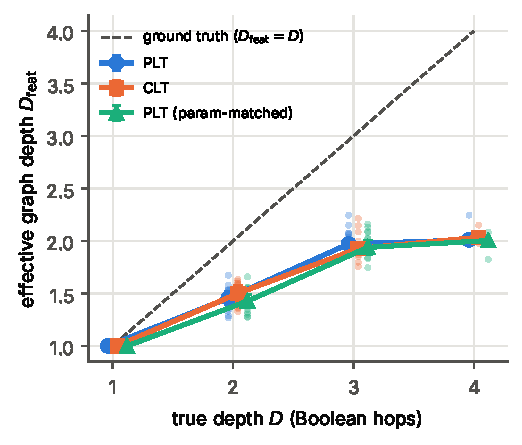
\includegraphics[width=0.45\linewidth]{figures/fig1_depth_vs_D.pdf}\\[4pt]
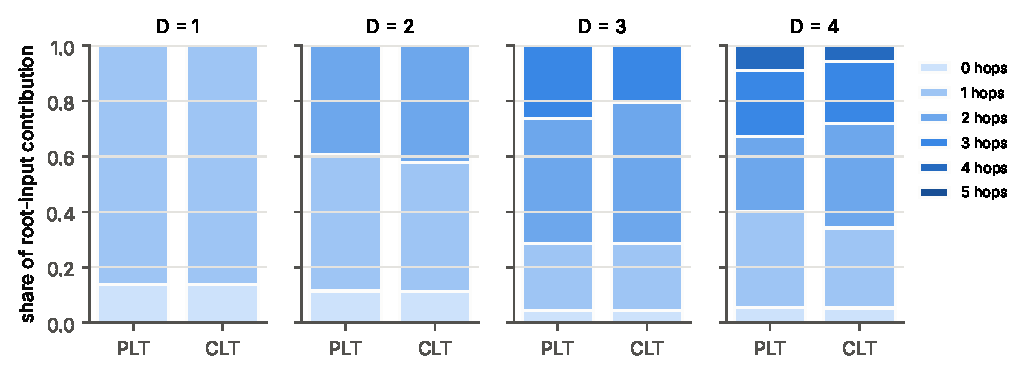
\includegraphics[width=0.95\linewidth]{figures/fig2_hop_profile.pdf}
\caption{Top: $\Dfeat$ vs.\ certified depth (dashed line: ground truth). Bottom: share of the root-input contribution by number of feature hops.}\label{fig:depth}\end{figure}
\paragraph{Both replacements reconstruct almost perfectly.} At the same budget, every replacement reaches relative MSE $\le\RelMSEMax$, and the full replacement model scores at least $\EtoEAccMin$ bit accuracy (Table~\ref{tab:fid}).
\paragraph{Both lose depth.} Graph depth grows with true depth, but much more slowly. At $D=3$, $\Dfeat=\DfeatCLTDThree$ for the CLT and $\DfeatPLTDThree$ for the PLT (DCR $\DCRCLTDThree$ and $\DCRPLTDThree$). At $D=4$ the DCR falls to $\DCRCLTDFour$ and $\DCRPLTDFour$ (Table~\ref{tab:depth}, Fig.~\ref{fig:depth}). Depth loss increases with $D$ for both replacement types (Spearman $\rho=\TrendRhoCLT$ for CLT, $\TrendRhoPLT$ for PLT).
\paragraph{At a matched budget, the headline depth gap is small.} The paired CLT$-$PLT difference in $\Dfeat$ is $\DiffCLTPLTDTwo$, $\DiffCLTPLTDThree$ and $\DiffCLTPLTDFour$ at $D=2,3,4$, with sign-flip $p=\PvalDTwo$, $\PvalDThree$ and $\PvalDFour$. The CLT does place more mass on edges that skip layers: $\SkipCLTDThree$ vs.\ $\SkipPLTDThree$ at $D=3$, and $\SkipCLTDFour$ vs.\ $\SkipPLTDFour$ at $D=4$.
% PILOT (3 seeds). Re-state after the full 5-seed run, the k-sweep and the param-matched PLT.

\section{What the Graphs Claim vs.\ What the Model Does}
\paragraph{The shortcuts are in the replacement, not the model.} Is the shallow graph a faithful picture of a model that takes logit-level shortcuts? Certification only checks the sign of the logit. We therefore measure $r_\mathrm{bypass}$: the mean $|\Delta\mathrm{logit}|$ when the upstream inputs and earlier sites are swapped while site $k$ is kept, relative to swapping site $k$ itself. In the original models $r_\mathrm{bypass}=\RbypassAllOrig$ on average, and the bypass swap never flips a decision. The \emph{replacement} models running the same test are far less bypass-free: $r_\mathrm{bypass}=\RbypassAllPLT$ for PLT and $\RbypassAllCLT$ for CLT, reaching $\RbypassPLTDThree$ and $\RbypassCLTDThree$ at $D=3$ (against $\RbypassOrigDThree$ for the original; not measured at $D=4$). They even flip up to $\BypassFlipMaxCLT$ of decisions. The CLT bypasses more than the PLT in $\NHopsCLTgtPLT$ of $\NHopsTotal$ (model, hop) pairs (Table~\ref{tab:bypass}). Accurate reconstruction on the data distribution therefore does not constrain counterfactual behaviour, and the depth the graph loses is introduced by the transcoders.
\begin{table}[t]\centering\caption{Logit-level bypass ratio $r_\mathrm{bypass}$ (lower = more faithful to the stepwise circuit).}\label{tab:bypass}\begin{tabular}{rrrr}\toprule
$D$ & original & PLT & CLT\\\midrule
2 & 0.060 & 0.107 & 0.108\\
3 & 0.042 & 0.148 & 0.321\\
\bottomrule\end{tabular}
\end{table}
\paragraph{Route freezing.} Freezing the CLT's cross-layer decoder writes at their base values leaves counterfactual accuracy at $\StepOnlyCLTDThree$ ($D=3$) and $\StepOnlyCLTDFour$ ($D=4$). Allowing \emph{only} the skip writes to update gives $\SkipOnlyCLTDFour$. The CLT's extra bypass therefore lives mostly in encoders that read upstream residual directions, not in its skip decoders.
\paragraph{How well the linearised graph predicts ablations.} The graph-predicted logit change from ablating a feature correlates with the actual change at $r=\AblRPLT$ for PLT but only $r=\AblRCLT$ for CLT (Fig.~\ref{fig:val}). CLT graphs are less faithful to their own replacement model.
\paragraph{Decodable is not causally used.} At the designated site, $\NAtSiteBoth$/$\NAtSite$ (point, hop) pairs are both decodable and causal. After the site, $\NAfterDecodable$ pairs are decodable and $\NAfterCausal$ are causal. \emph{Before} the hop is computed, $\NBeforeDecodable$ pairs are already decodable, because an AND of available inputs is linearly separable, yet $\NBeforeDecodableCausal$ are causal (1000-permutation probes; smallest $p=\MinPermP$).
\begin{figure}[t]\centering
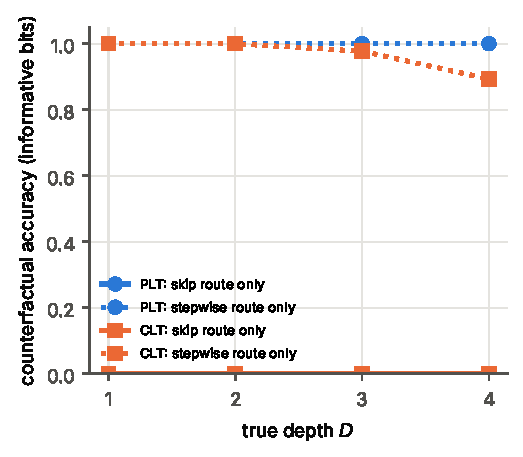
\includegraphics[width=0.48\linewidth]{figures/fig4_skip_dependence.pdf}\hfill
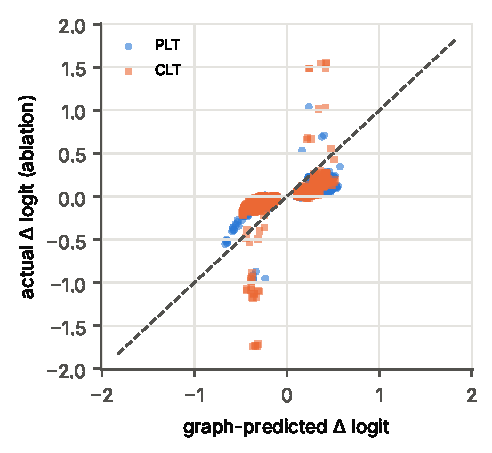
\includegraphics[width=0.44\linewidth]{figures/fig5_ablation_check.pdf}
\caption{Left: counterfactual accuracy when only the skip route or only the stepwise route may update. Right: graph-predicted vs.\ actual effect of ablating a feature.}\label{fig:val}\end{figure}

\section{Validation on a Pretrained Language Model}\label{sec:realdata}
% Every number below is a macro from generated/numbers_lm.tex (scripts/make_lm_tables.py).
% Write the interpretation sentences ONLY after the Colab run; state the result whichever way it goes.
A controlled Boolean setting establishes correctness but may make attribution too easy. We therefore apply the
identical pipeline (matched-budget PLT and CLT, feature-to-feature graphs with error nodes, the same depth
metric) to two-hop factual recall in \LMModel{}~\cite{lindsey2025biology}:
\emph{``Fact: the capital of the state containing Dallas is''} $\to$ \emph{Austin}. The intermediate entity
(\emph{Texas}) is known, and a one-hop control prompt with the same answer
(\emph{``Fact: the capital of Texas is''}) removes exactly one inferential step. We keep prompts whose answer
ranks in the model's top ten and whose state capital the model also knows, leaving \LMNTwoHop{} two-hop and
\LMNOneHop{} one-hop prompts. Both transcoders use the same features per layer, TopK $k$, steps, data and seed;
held-out normalised MSE is \LMNMSEPLT{} (PLT) and \LMNMSECLT{} (CLT).

\paragraph{V1: is the depth metric sensitive to depth on real data?}
If $\Dfeat$ measures inferential depth, it should be larger from the city tokens of a two-hop prompt than from
the state tokens of its one-hop control. Paired by state, $\Dfeat(\text{2-hop})-\Dfeat(\text{1-hop})$ is
\LMVOnePLT{} [\LMVOneLoPLT{}, \LMVOneHiPLT{}] for the PLT ($p=\LMVOnePPLT$) and
\LMVOneCLT{} [\LMVOneLoCLT{}, \LMVOneHiCLT{}] for the CLT ($p=\LMVOnePCLT$).

\paragraph{V2: are the state features causally used?}
State-selective features are chosen leave-one-out, so the prompt being tested never influences the selection.
Zeroing them lowers the answer logit by \LMVTwoPLT{} [\LMVTwoLoPLT{}, \LMVTwoHiPLT{}] (PLT) and
\LMVTwoCLT{} [\LMVTwoLoCLT{}, \LMVTwoHiCLT{}] (CLT) \emph{more} than zeroing the same number of random active
features in the same layers ($p=\LMVTwoPPLT$, $p=\LMVTwoPCLT$).

\paragraph{V3: does the graph's claim match the intervention?}
Across prompts, the graph-claimed mediation through state features (IMF) correlates with the measured ablation
drop with Spearman $\rho=\LMVThreePLT$ (PLT, $p=\LMVThreePPLT$) and $\rho=\LMVThreeCLT$ (CLT, $p=\LMVThreePCLT$).

\paragraph{V4: CLT versus PLT.}
On the same two-hop prompts, CLT minus PLT $\Dfeat$ is \LMDfeatDiffCLTminusPLT{} ($p=\LMDfeatDiffP$);
Table~\ref{tab:lm} reports skip mass, IMF, ablation drop and error influence.

% AUTO-GENERATED by scripts/make_lm_tables.py
\begin{table}[t]\centering\scriptsize
\caption{Real-data validation on two-hop factual recall. Mean [95\% bootstrap CI]; sign-flip $p$.}\label{tab:lm}
\begin{tabular}{llp{3.6cm}ll}\toprule
Test & Kind/hop & Quantity & Mean [CI] & $p$ (n)\\\midrule
V1 depth sensitivity & clt & D feat(2hop) - D feat(1hop), per state & 0.09 [-0.06, 0.22] & 0.344 (n=6)\\
V1 depth sensitivity & clt & abs-normalised D feat(2hop) - D feat(1hop), per state & -0.02 [-0.04, 0.00] & 0.219 (n=6)\\
V2 causal specificity & clt & logit drop: state features - random features & 4.33 [2.27, 6.52] & 0.016 (n=7)\\
V3 graph vs intervention & clt & Spearman(IMF, ablation drop) & 0.64 [--, --] & 0.119 (n=7)\\
V1 depth sensitivity & plt & D feat(2hop) - D feat(1hop), per state & 0.28 [0.17, 0.38] & 0.031 (n=6)\\
V1 depth sensitivity & plt & abs-normalised D feat(2hop) - D feat(1hop), per state & -0.13 [-0.20, -0.07] & 0.031 (n=6)\\
V2 causal specificity & plt & logit drop: state features - random features & 0.83 [-0.85, 2.93] & 0.594 (n=7)\\
V3 graph vs intervention & plt & Spearman(IMF, ablation drop) & 0.57 [--, --] & 0.180 (n=7)\\
V4 clt minus plt & 2hop & root signed D feat & -0.16 [-0.35, -0.02] & 0.059 (n=10)\\
V4 clt minus plt & 1hop & root signed D feat & -0.03 [-0.15, 0.09] & 0.608 (n=12)\\
V4 clt minus plt & 2hop & skip mass & 0.07 [0.07, 0.08] & 0.002 (n=10)\\
V4 clt minus plt & 1hop & skip mass & 0.06 [0.05, 0.06] & 0.000 (n=12)\\
V4 clt minus plt & 2hop & IMF h1 & 0.04 [0.01, 0.08] & 0.047 (n=10)\\
V4 clt minus plt & 2hop & state ablation logit drop & 0.72 [-0.08, 1.64] & 0.188 (n=10)\\
V4 clt minus plt & 2hop & error influence & -0.08 [-0.09, -0.07] & 0.002 (n=10)\\
V4 clt minus plt & 1hop & error influence & -0.07 [-0.08, -0.06] & 0.000 (n=12)\\
\bottomrule\end{tabular}\end{table}


\paragraph{Scope.} The real-model transcoders are trained by us at a matched budget but are far smaller than
production transcoders; error nodes carry \LMErrInflPLT{} (PLT) and \LMErrInflCLT{} (CLT) of the logit's
influence, and the replacement model without error terms keeps the original top-1 token on a fraction
\LMTopKeptPLT{} (PLT) and \LMTopKeptCLT{} (CLT) of prompts. InterpBench~\cite{gupta2024interpbench}
(semi-synthetic SIIT transformers with known circuits) is the natural next step between our certified
Boolean models and a pretrained LM; the evaluation code is included but was not run for this submission.

\section{Limitations and Conclusion}
Our models are semi-synthetic. Certification makes their depth precise, but it relies on interventions we chose (see docs/threats\_to\_validity.md). Backup computation in non-circuit components can make the full model's graph shallower without any transcoder artefact. We control for this by pairing PLT and CLT on the same base models. With five seeds per depth, per-depth tests cannot reach $p<0.05$; we rely on pooled trend tests and confidence intervals. The real-model tiers use pruned graphs, and we report their coverage.
% Conclusion: write after the full run.

\IfFileExists{splncs04.bst}{\bibliographystyle{splncs04}}{\bibliographystyle{plain}}
\bibliography{refs}
\end{document}
